\blankpage

\thispagestyle{empty}
\clearpage
\begin{tikzpicture}[remember picture, overlay]
\node at (3,-7) {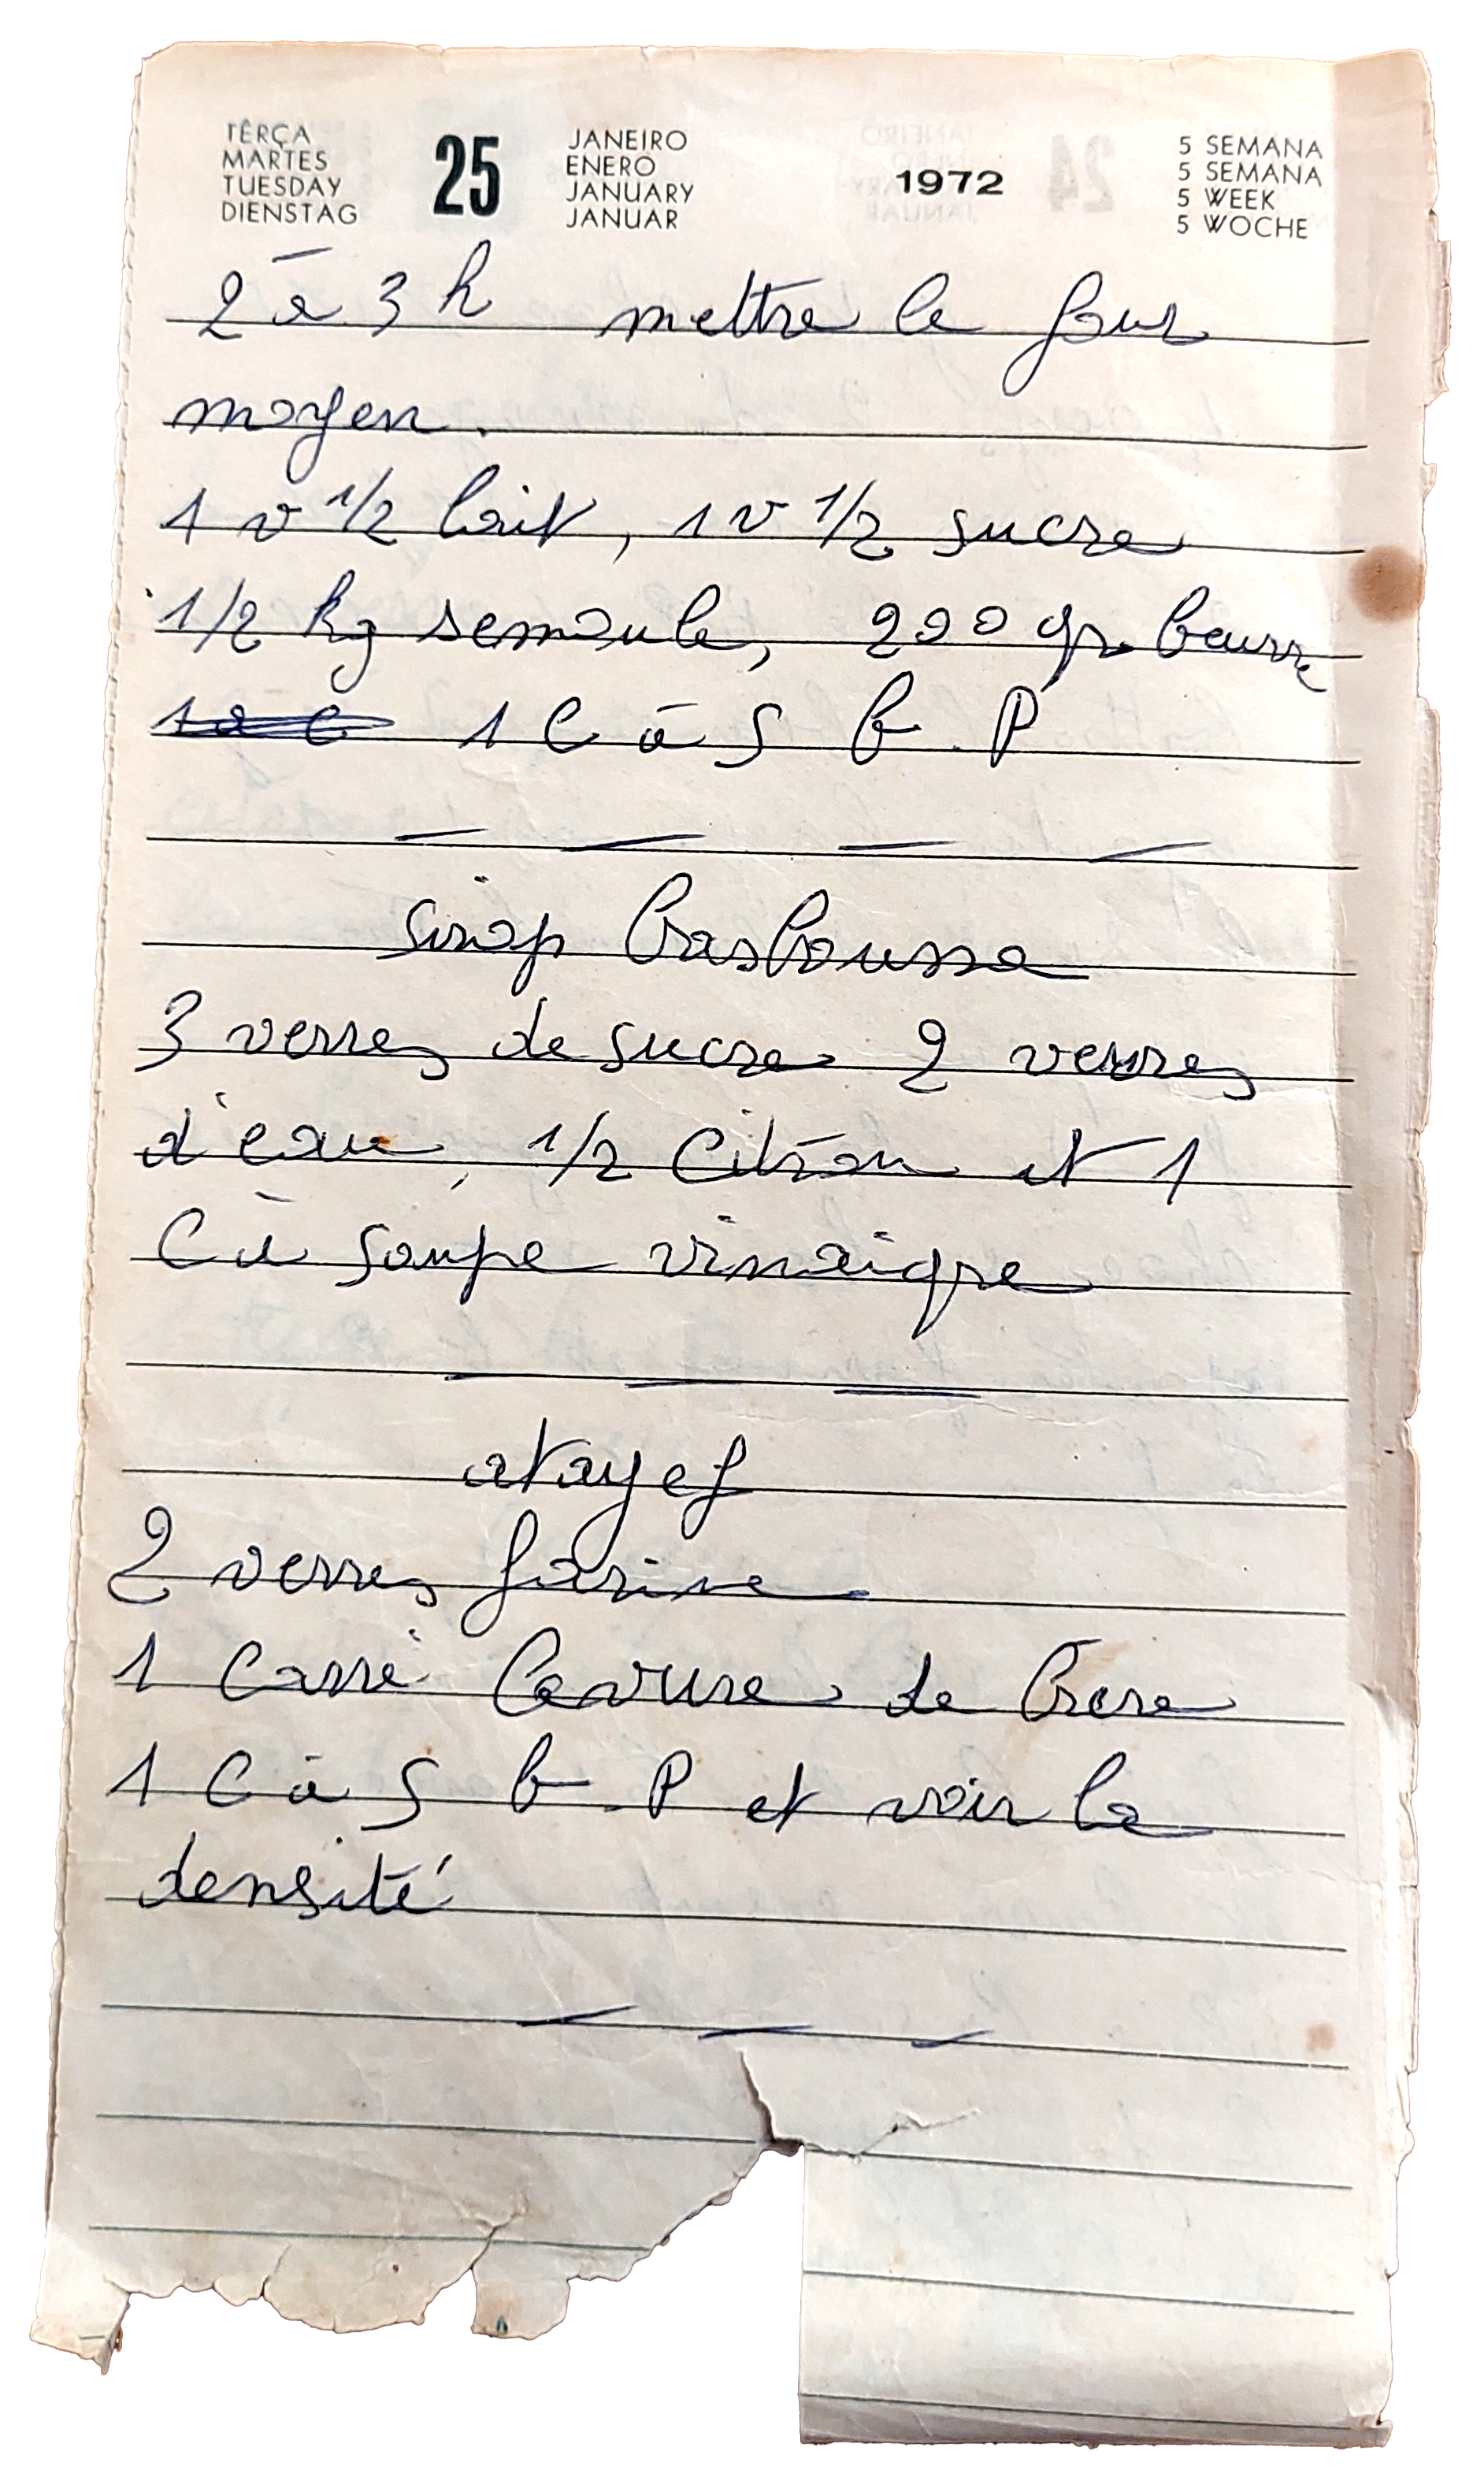
\includegraphics[width=8cm]{./recettes/edités/Gateau choc Ziza, Basboussa et Atayef (parte 2).jpg}}; 
\end{tikzpicture}\clearpage\thispagestyle{empty}
% \begin{tikzpicture}[remember picture,overlay]
% \fill[black] (-3,3.5) rectangle (14,-21.5);
% \end{tikzpicture}
\clearpage

\chapter*{Atayef}

\section{Ingrédients originaux}

\begin{itemize}
\item 2 verres farine
\item 1 case levure de bière
\item 1 c à s B.P et voir la densité
\end{itemize}

\section{Préparation adaptée}

Mélangez la farine avec la levure de boulanger et la levure chimique (\textsc{b.,p.}), puis ajoutez de l’eau tiède jusqu’à obtenir une pâte lisse, semi-liquide. Laissez reposer 30--60 minutes jusqu’à formation de bulles. Versez de petites portions dans une poêle chaude sans matière grasse et faites cuire d’un seul côté jusqu’à ce que la surface soit trouée et sèche. Laissez refroidir, puis garnissez de noix hachées mélangées avec du sucre et un peu d’eau de fleur d’oranger, et repliez en demi-lune.

\chapter{Atayef}

\section{Ingredientes originais}

\begin{itemize}
\item 2 copos de farinha
\item 1 tablete de fermento biológico
\item 1 colher de sopa de B.P. e ver a densidade
\end{itemize}

\section{Modo de preparo adaptado}

Misture a farinha com o fermento biológico e o fermento químico (\textsc{b.,p.}), depois adicione água morna até obter uma massa lisa e semilíquida. Deixe descansar por 30--60 minutos, até formar bolhas. Despeje pequenas porções em uma frigideira quente sem untar e cozinhe de um só lado, até que a superfície esteja cheia de furinhos e seca. Deixe esfriar, depois recheie com nozes picadas misturadas com açúcar e um pouco de água de flor de laranjeira, e feche em meia-lua.